\chapter{M-ary modulation schemes}
\label{mary}
In the following programs, I've implemented a general M-ary shift keying modulator.
So to get 4-ary modulation (or 8-ary) just set $M$ = 4 (or $M$ = 8) in the program.

\section{Context}
An M-ary modulation means, for modulating quantity, M different level are used for transmitting M symbols.
\begin{itemize}
	\item in M-ary FSK: M different frequencies are used.
	\item in M-ary PSK: M different phases are used.
	\item in M-ary ASK: M different amplitudes are used.
\end{itemize}

Usually all these modulated quantities are equally spaced.

When a bit sequence is given, they have to be grouped and converted to equivalent decimal format to do rest of modulation.
For M-ary modulation, number of bits in each group is $n = log_2(M)$.
If Enough bits are not there (ie we have to group every 2 bits, but there're only 5 bits), additional zeros has to added. For eg. grouping in 4-ary will be:

00101 -> 00 10 10 (grouping of 2 bits)

and in 8-ary:

00101 -> 001 010 (grouping of 3 bits)

Where the zero should be added?
It cab be added in either front or back of the sequence, as long as you can create a demodulate scheme which discards this extra zero.
(in this case I've added it at the end of each group).

\section{M-ary ASK}
Generally for M signals, M different amplitude levels should be used.
For eg. in QASk, 4 equally spaced amplitude levels will be used. In practice, it can be of any value: [1 2 3 4] or [-3 -1 1 3], etc...

In my implementation, I created amplitude levels corresponding to each decimal digit $d$ which ranges from 0 to $M-1$ by interpolating $d$ to range from $L_{min}$ to $L_{max}$
(which corresponds to minimum and maximum amplitude level). Hence amplitude corresponds to decimal digit $d$ is

$$\therefore \text{amplitude(d)} = \frac{d}{M-1} * (L_{max} - L_{min}) + L_{min}$$

\subsection*{Program}
\setstretch{1}
\importMLCode{code/mary.m}
\setstretch{1.15}
The length of sequnce has to be adjusted in such a way that grouping is possible. for 4-ary, input length should be multiple of 2, for 8-ary, input length should be multiple of 3, and so on..

To do such adjustment, some number of bits should be added. The following code checks if input length is multiple of $n$ and if not, it adds required number of zeros.
\begin{minted}[frame=single]{matlab}
if mod(length(x), n) ~= 0
    x = [x, zeros(1, n - mod(length(x), n))];
end
\end{minted}

for eg.: if n = 3 (for 8-ary modulation), and input length is 7, {\tt mod(7, 3) = 1}, hence 3 - 1 = 2 more zeros are added.

\begin{figure}[ht!]
	\centering
	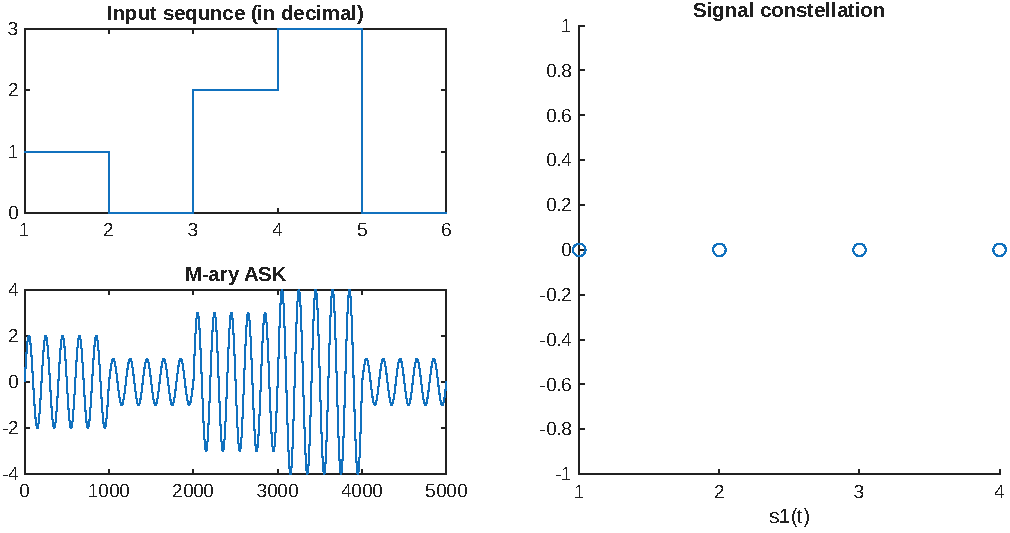
\includegraphics[width=\textwidth]{img/mask.pdf}
\end{figure}


\section{M-ary PSK}
M-ary here divides phases from 0 to $2\pi$ into M intervals.
If each group of bits corresponds to digit d. Then corresponding M-PSK signal is:
$$s(t) = A_c \sin\left(2 \pi f_c t + \frac{2\pi}{M} d\right)$$

Where $d$ can take valus either from 0 to $M-1$ or 1 to $M$. Notice that in this representation the signal constellation will contain a signal vector at $0^\circ$. This signal vector at $0^\circ$ can be avoided by adding additional phase shift of $\pi / M$ to whole signal. This is illustrated in following:
\\[10pt]
\begin{figure}[!ht]
	\begin{minipage}[t]{.45\textwidth}
		\centering
		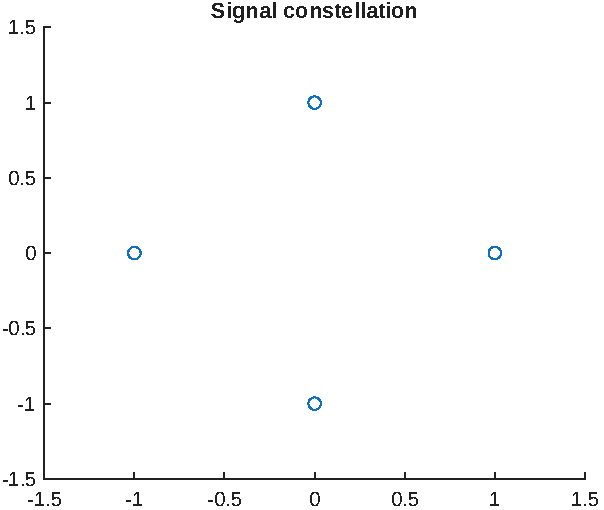
\includegraphics[width=\linewidth]{img/0ps.pdf}
\\[10pt]
		With signal vector at $0^\circ$ \\[5pt]
		$s(t) = A_c \sin\left(2 \pi f_c t + \dfrac{2\pi}{M} d\right)$
	\end{minipage}\hfill%
	\begin{minipage}[t]{.45\textwidth}
		\centering
		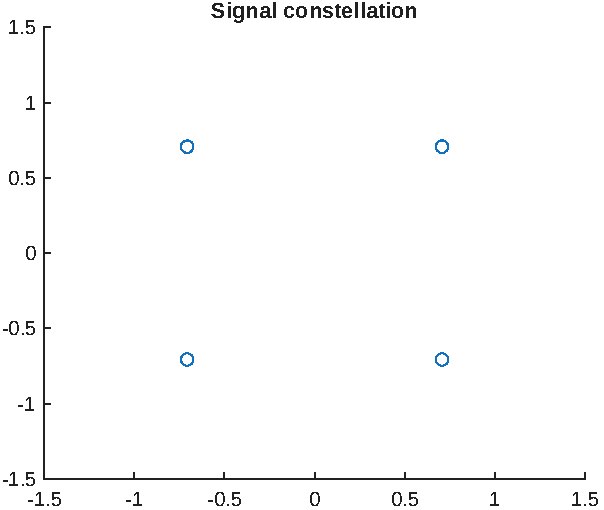
\includegraphics[width=\linewidth]{img/ps.pdf}
\\[10pt]
		No signal vector at $0^\circ$ \\[5pt]
		$s(t) = A_c \sin\left(2 \pi f_c t + \dfrac{2\pi}{M} d + \dfrac{\pi}{M}\right)$
	\end{minipage}
\end{figure}

\subsection*{Program}
Here I've implemented a modulator that doesn't produce signal vector at $0^\circ$ phase shift. Here's how it is implemented:

I've expressed all signals in complex form, this allows phase shift to be applied to signals by just multiplying by another complex number.
The carrier signal is written in complex form:
$$c(t) = A_c\exp\left(j2\pi f_c t\right)$$

Phase shift for a partial symbol $d$ is:
\begin{equation}
	\text{phase}(d) = \exp\left[j\left(2\pi \dfrac{d}{M} + \dfrac{\pi}{M}\right)\right]
	\label{phased}
\end{equation}

Hence signal corresponding to given decimal $d$ is:
\begin{align*}
	s(t) &= c(t) \cdot \text{phase}(d) \\
&= A_c\exp\left(j2\pi f_c t\right) \exp\left[j\left(2\pi \dfrac{d}{M} + \dfrac{\pi}{M}\right)\right] \\[5pt]
\Aboxed{s(t)&= \exp\left[j\left(2\pi f_c t + 2\pi \dfrac{d}{M} + \dfrac{\pi}{M}\right)\right]}
\end{align*}

To plot the signal, either real or imaginary part of $s(t)$ can be taken.
If imaginary part is taken:

$$\mathfrak{Im}(s(t)) = A_c\sin\left[2\pi f_c t + 2\pi \dfrac{d}{M} + \dfrac{\pi}{M}\right]$$

NOTE: in the program, $A_c$ is taken as 1.
\importMLCode{code/mpsk.m}

\begin{figure}[!ht]
	\centering
	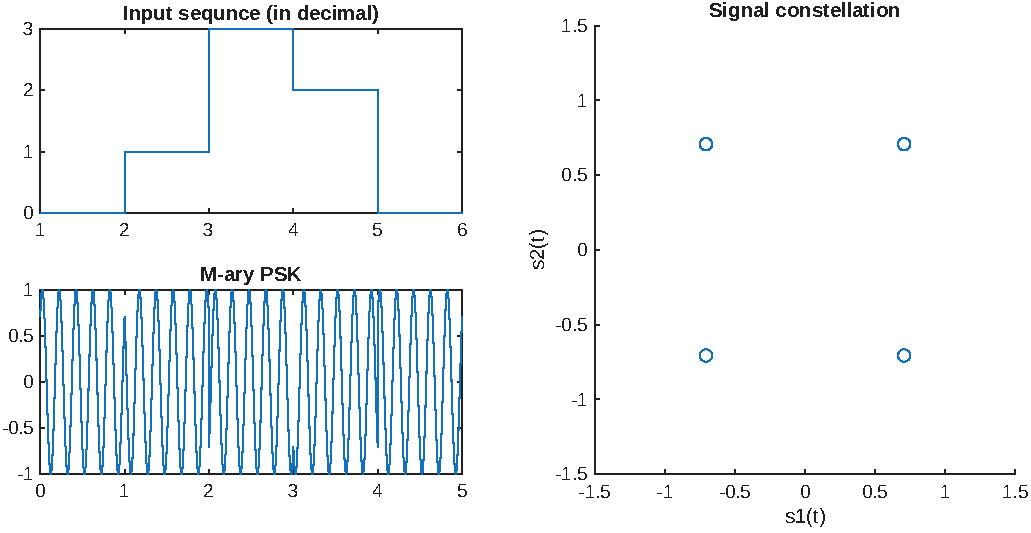
\includegraphics[width=\linewidth]{img/mpsk.pdf}
\end{figure}

The signal constellation will have axis which are orthonormal basis functions used in PSK. 
Here, I've used \textit{orthogonal} signals: $s1(t) = \cos(2\pi f_c t)$ and $s2(t) = \sin(2\pi f_c t)$
which are real and imaginary component of phase(d) in Eq. \ref{phased}.

The case illustrated above is 4-ary. If you want to plot constellation for 8-ary, appropriate message bit stream must be provided, that generates signals of all phases (this is true for all other modulation schemes)

\section{M-ary FSK}

In the same way, M-ary FSK will have M different frequencies: $$f_c, \quad f_c + \Delta f, \quad f_c + 2\Delta f, \quad \cdots, \quad f_c + (M-1)\Delta f$$

Where $\Delta f$ is the distance between each frequency.

Hence for each decimal digit $d$ corresponding to some group of binary, signal is given by:

$$s(t) = \sin\left(2\pi (f_c + d \Delta f) t\right)$$

\section*{Program}
\importMLCode{code/mfsk.m}
\begin{figure}[!ht]
	\centering
	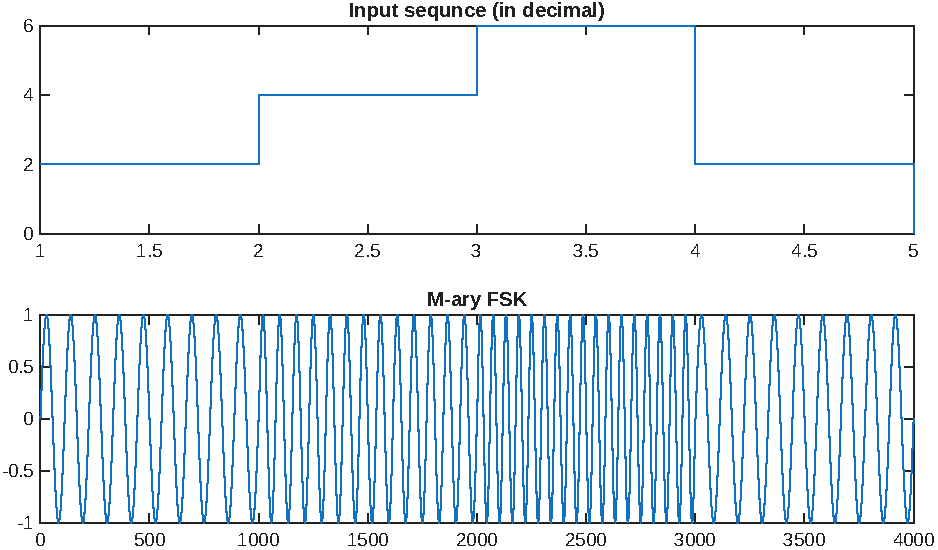
\includegraphics[width=0.8\linewidth]{img/mfsk.pdf}
\end{figure}

The signal constellation of M-ary FSK will have M-dimensions, which is hard to visualize for 4-ary or 8-ary FSK.

\section{BER vs SNR, Signal constellation}
The following is an example for BER(Bit error rate) or Symbol error rate (for M-ary modulation) vs SNR plot of BPSK and QPSK. BER is ratio of number of wrong symbols detected after demodulation to total number of symbols. Usually its a small number hence it is expressed in log scale:

$$\text{BER} = 10\log_{10} \left(\frac{\text {No. of incorrectly decoded symbols}}{\text{Total no. of symbols}}\right)$$

The errors can happen due to noise in the channel.
This noise is simulated by using function \texttt{awgn(x, snr)} .
This function adds noise to input $x$ in such a way that the output SNR is as given to it.
Hence to obtain BER at a given \texttt{snr} following steps are done: (this is same for any modulation scheme)
\begin{enumerate}
	\item Modulate signal $x(n)$ and obtain $m(t)$ (modulated wave)
	\item apply noise: \mintinline{matlab}{y = awgn(x, snr)} 
	\item demodulate it, and get $d(n)$
	\item Count number of symbol errors (using \mintinline{matlab}{sum(x ~= d)})
\end{enumerate}

{\setlength{\parindent}{0pt} Use a loop to find BER for a range of SNRs}

\subsection*{Program}
This uses matlab's built in \mintinline{matlab}{pskmod} and \mintinline{matlab}{pskdemod} functions.


\importMLCode{code/psk_ber.m}

\begin{figure}[!ht]
	\centering
	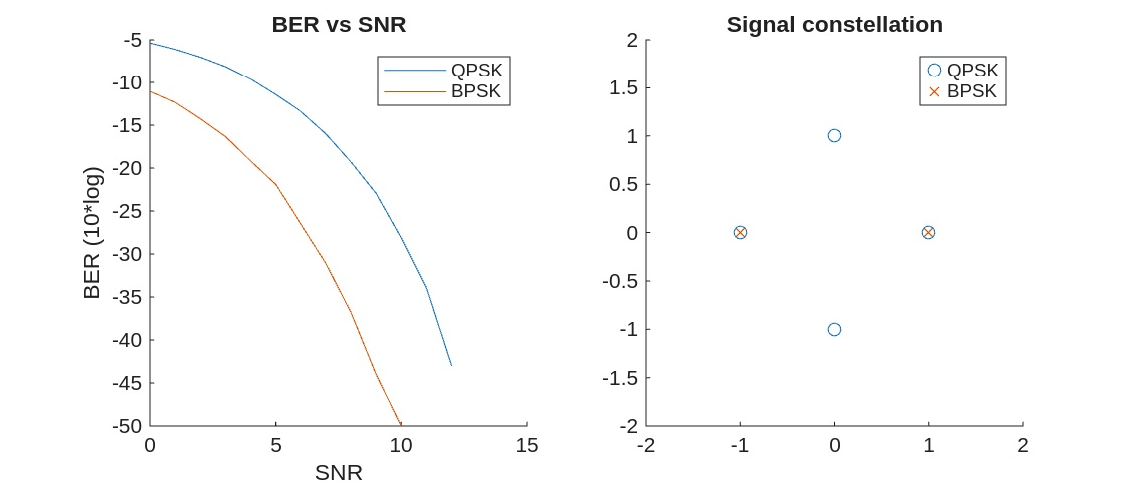
\includegraphics[width=\linewidth]{img/psk_props.pdf}
\end{figure}

\begin{tcolorbox}[breakable, title=More on Matlab's build-in modulators \& demodulators]
	In my implementation, I took a bit sequence and converted it to decimal to do any useful operation. However MATLAB's build in functions only takes decimal values. The modulation also works differently (for eg: in case of PSK, matlab uses gray codes to map each input to corresponding phase value, also it uses different set of phase differences). If you try with PSK, you'll get following points: 
\begin{minted}[frame=single]{matlab}
>> pskmod([0 1 2 3], 4)
ans =
1.0000 + 0.0000i
0.0000 + 1.0000i
-0.0000 - 1.0000i
-1.0000 + 0.0000i

>> pskmod([0 1 2 3 4 5 6 7], 8)
ans =
1.0000 + 0.0000i
0.7071 + 0.7071i
-0.7071 + 0.7071i
0.0000 + 1.0000i
0.7071 - 0.7071i
-0.0000 - 1.0000i
-1.0000 + 0.0000i
-0.7071 - 0.7071i
\end{minted}

This is visualised as following: (notice that grey code is assigned in clockwise manner)

\begin{minipage}[t]{\textwidth}
		\centering
		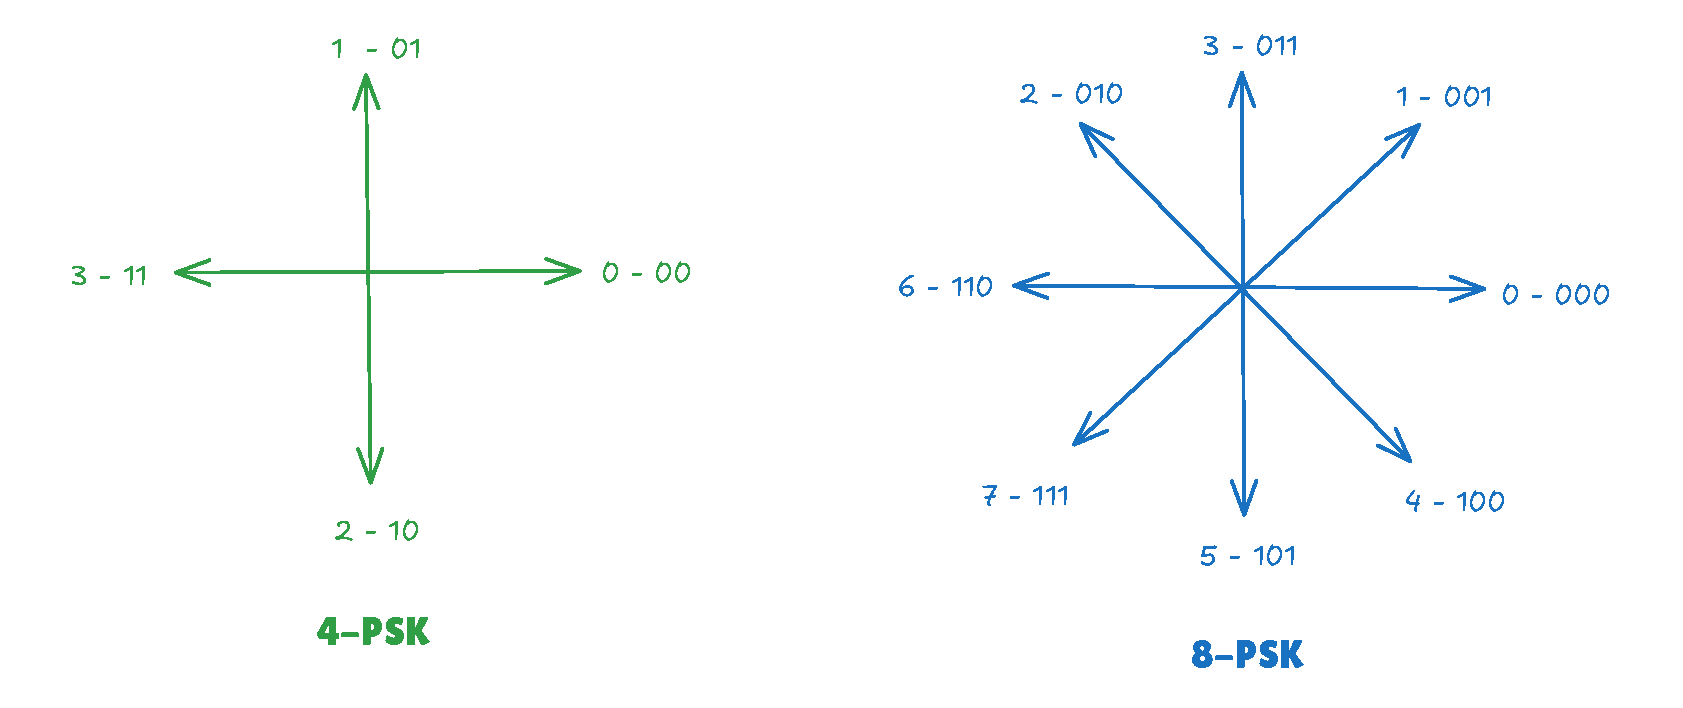
\includegraphics[width=0.9\linewidth]{img/psk_diag.pdf}
\end{minipage}

Subsequently, the demodulation also produces integer sequence corresponding to each modulated vector.

\begin{minted}[frame=single]{matlab}
>> pskdemod([1, i, -i, -1], 4)
ans =
0     1     2     3
\end{minted}

Similarly there is \texttt{fmmod} and \texttt{fmdemod} functions for FM modulation. More on it here:
\href{https://in.mathworks.com/help/comm/ref/fmmod.html}{https://in.mathworks.com/help/comm/ref/fmmod.html}
	
\end{tcolorbox}
